\begin{figure}[t!]
    \begin{center}
        \begin{subfigure}{0.49\textwidth}
            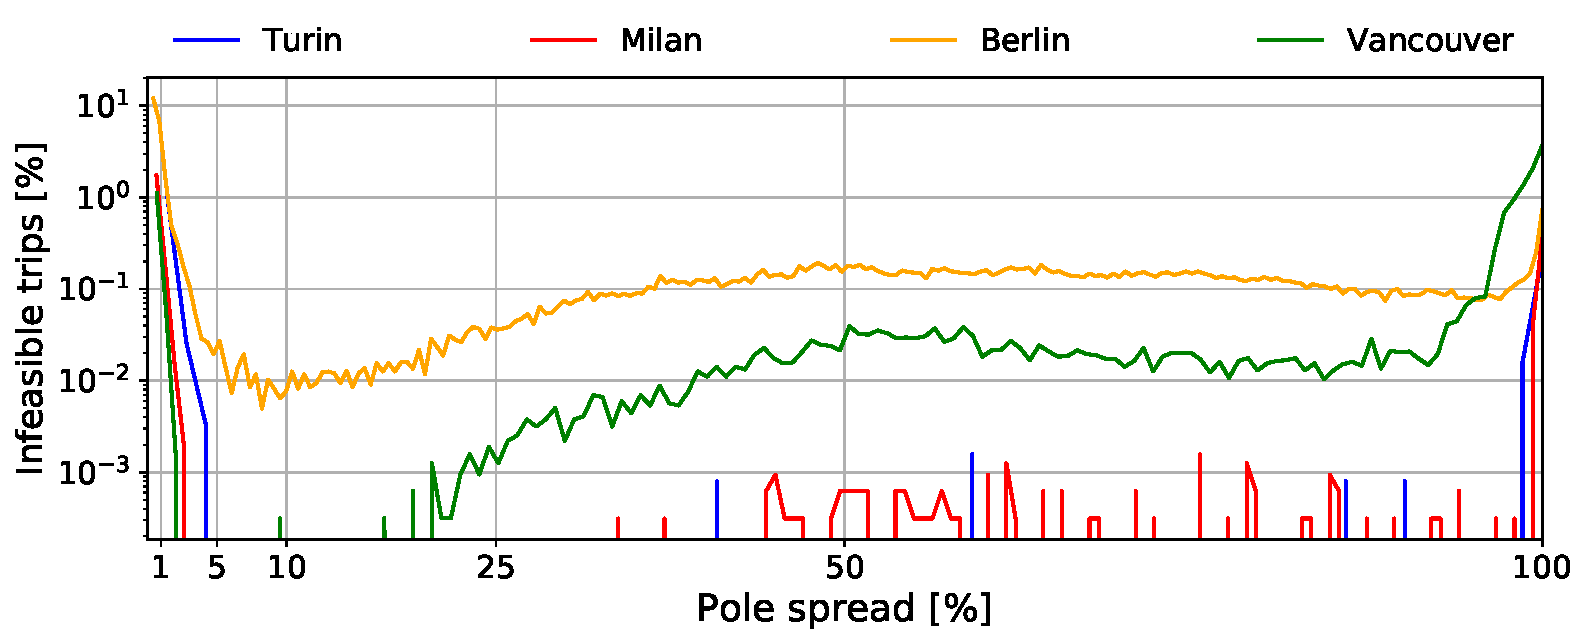
\includegraphics[width=\columnwidth]{figures/50_Deaths_vsZones_ACS}
            \caption{Infeasible trips - the lower the better.}
            \label{fig:zoneACS_vs_IT}
        \end{subfigure}
                  \begin{subfigure}{0.49\textwidth}
            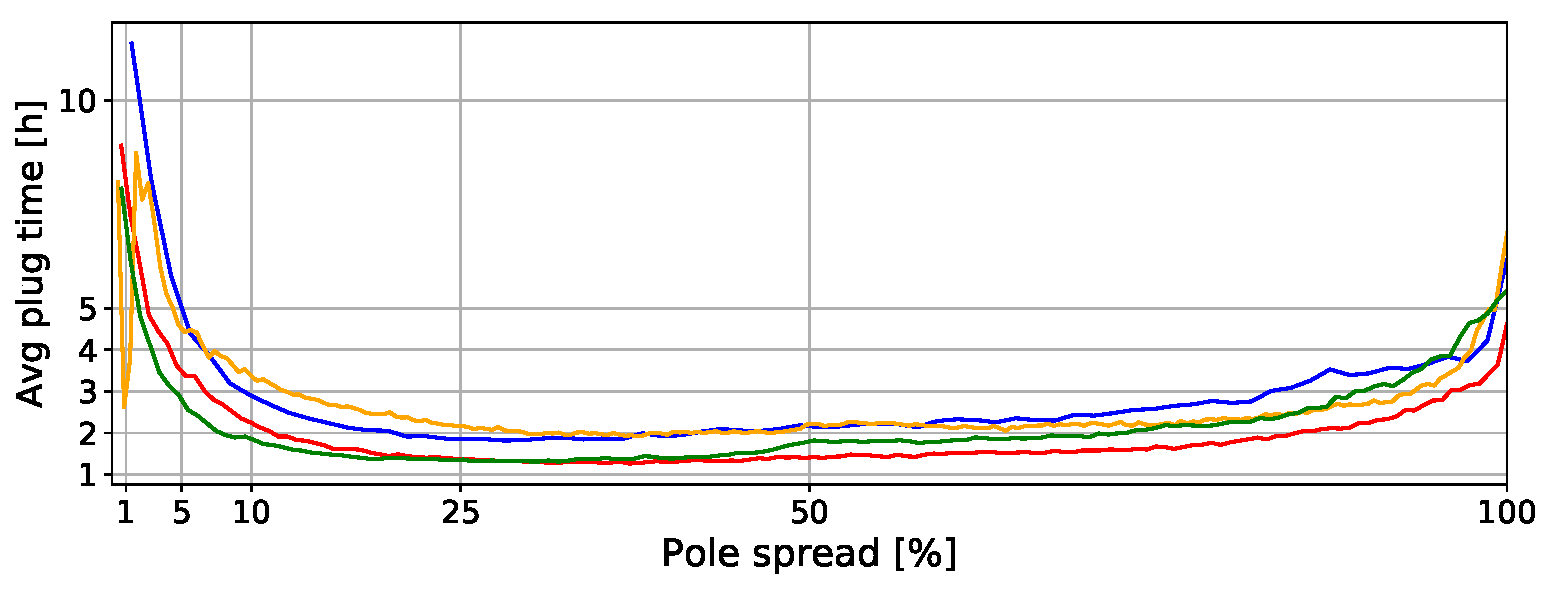
\includegraphics[width=\columnwidth]{figures/50_AvgTimeInStation_vsZones_ACS.pdf}
             \caption{Average time spent plugged to a pole.}
             \label{fig:zoneACS_vs_plug}
         \end{subfigure}        
           \begin{subfigure}{0.49\textwidth}
            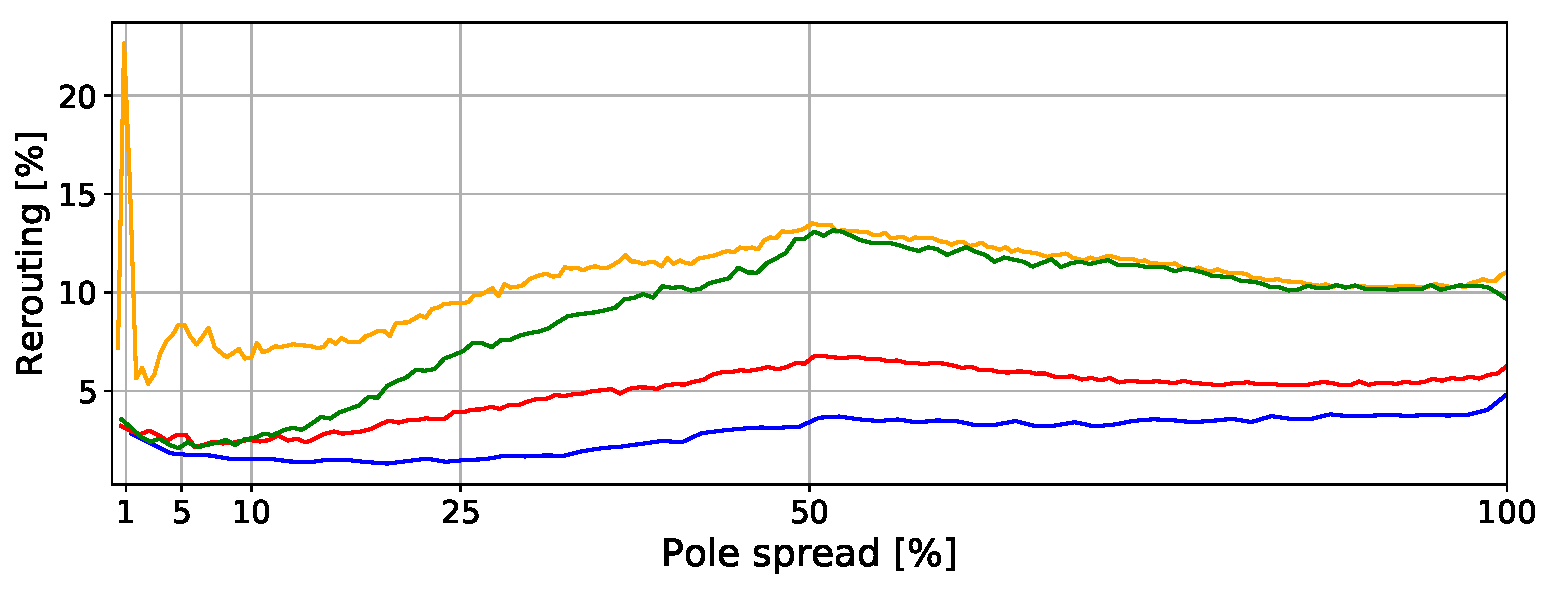
\includegraphics[width=\columnwidth]{figures/50_ReroutePerc_vsZones_ACS}
             \caption{Reroute events percentage - the lower the better.}
             \label{fig:zoneACS_vs_Reroute}
         \end{subfigure}        
         \begin{subfigure}{0.49\textwidth}
            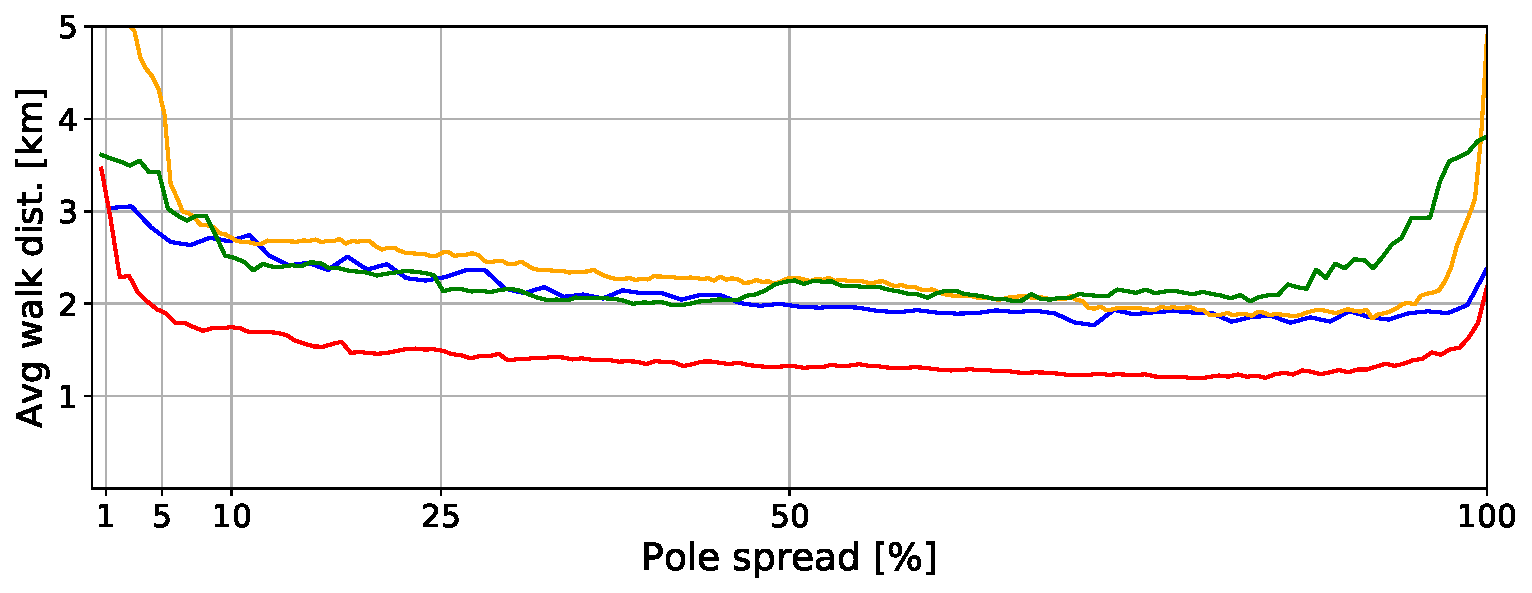
\includegraphics[width=\columnwidth]{figures/50_AvgWalkedDistance_vsZones_ACS.pdf}
             \caption{Average walk distance for rerouted trips - the lower the better.}
             \label{fig:zoneACS_vs_awd}
         \end{subfigure}
         \caption{Impact of pole distribution among zones. Concentrating all poles in very few hubs performs poorly, as well as placing single pole charging stations.}
         \label{fig:zoneACS}
\end{center}
\end{figure}

\section{How to distribute poles in stations}
\label{sec:resPoles}

In the previous sections, we have assumed charging stations with $k=4$ poles each. Here, we study the impact of installing charging station with a larger or smaller number of poles each. We keep the total number of charging poles $K=kN$ constant, and equally distribute them in a varying number of charging stations $N$. In other words, we check if it is better to have (i) big charging hubs with many poles (one single hub corresponds to $N=1$, with $K$ poles), or (ii) a very large number of charging stations each with one pole ($N=K$, $k=1$).
We call {\it pole spread percentage} the percentage of zones in which poles are distributed among, i.e., $100N/K = 100/k$. For example, pole spread percentage 5 corresponds to 20 poles per zone ($k=20$), spread percentage 10 corresponds to 10 poles per zones, etc. up to spread 100 that corresponds to a single pole per each charging zone ($N=K$ and $k=1$).

For each of the four cities we pick a constant number of charging poles $K$, corresponding to a percentage of 7\% of charging zones when $k=4$.\footnote{Each city has a different $K$, producing a different number of infeasible trips.} Then, we distribute the poles evenly among different numbers of $N$ zones, chosen according to the highest number of parkings (as in the previous Sections). 
We consider the Hybrid policy with $w=0.5$ and simulate the  resulting system. 

From top to bottom, Fig.~\ref{fig:zoneACS} reports percentage of infeasible trips, the average time cars are plugged to a charging pole (even if they are completely charged), the percentage of rerouted trips,  and the average walk distance for rerouted trips. 
Colors refer to different cities and the x-axis reports the spread percentage. 
%For instance the leftmost point corresponds to a single hub where all $K$ poles are located. The rightmost point corresponds to having $N=K$ zones, each with a single pole. 
%Dots highlight those fraction for which all zones have the same number of poles, i.e., where $(K/N)=k \,\land\, mod(K,N)=0$. 
Note that with $k=4$, as in the previous experiments, we have a spread percentage of 25\% for all the cities.

%Results are striking. 

Focus first on Fig.~\ref{fig:zoneACS_vs_IT}. With spread percentage going below 5\%, hence concentrating poles in very few hubs, the number of infeasible  trips quickly grows to non negligible values. Even Turing and Milan suddenly suffer of a sizable percentage of infeasible trips.
The lowest values are obtained with spread between 5 and 20, meaning that increasing the number of poles per charging station in the $[5-20]$ range helps the system to sustain.
For instance, placing stations with $k=6$ poles lets Vancouver sustain all trips. 
Conversely, spreading a lot of charging stations, each equipped with one pole is also not optimal. Poles are occupied for long time by cars that customers tend to not rent, since located in non-popular areas, as can been seen by the (too) high plugged time in Fig.~\ref{fig:zoneACS_vs_plug}.

%Fig.~\ref{fig:zoneACS_vs_plug} shows the average time spent plugged to a charging station, during a charge event.

Fig.~\ref{fig:zoneACS_vs_Reroute} shows the percentage of reroutings. Here we also observe that it is better to have a low spread percentage.
For the region where we have negligible infeasible trips (spread between 5 and 20), the percentage of reroutings increase both because poles start to be located in less popular destination, and because cars are charged for less time (see Fig.~\ref{fig:zoneACS_vs_plug}).

Lastly, we show walk distance for rerouted trips in Fig.~\ref{fig:zoneACS_vs_awd}. As expected, the walk distance slowly decreases with spread percentage. Indeed, when customers are rerouted, they can return the cars in more areas, likely closer to their desired destination. Only when single poles are used, the walk distance increases again. This is justified by cars that stay attached to poles for (too) long time, reducing the availability of free poles, thus forcing customers to drive further away.

%First, concentrating poles in few hubs performs poorly. In all cities, the infeasible trips suddenly grow by one or more order of magnitude as seen in Fig.~\ref{fig:zoneACS_vs_IT} (note the log y-scale). 

%This inefficiency is due to several effects: 
%(i) Since customers rent cars in the closest zone from their actual position, they tend to pick cars that are freely parked in the city area, and not those cars parked in the hub. 
%(ii) As such, a lot of cars stay connected for long time at the poles in the hub -- see Fig.~\ref{fig:zoneACS_vs_ACS}. This reduces the number of free poles.
%(
%(ii) When a car needs to be charged ($c(a,t)<\pi)$), there is a sizable probability of having all poles being busy - thus making it impossible to charge the car. 

%. A such, the number of available poles is smaller, rerouting customers far away (Fig.~\ref{fig:zoneACS_vs_awd}), and increasing the chance to run out of battery (Fig.~\ref{fig:zoneACS_vs_IT}).

Therefore, the best trade-off is hard to detect and depends from city to city. 
%obtained with spread factors $k\in[5,10]$, 
In general, it looks better to concentrate poles only in those zones where cars are frequently rented and returned, so to increase the chance to find a free pole, and let the battery quickly charge before the next rental makes the pole free again. %Infeasible trips are thus minimized. The only drawback is the high walk distance in case of rerouting (Fig~\ref{fig:zoneACS_vs_awd}). As previously suggested, the impact of this could be reduced by adopting some relocation policy, and giving incentives to customers.

Note that both extreme solutions of pole spread percentage would also cause the highest installation and operating expenditures. The single hub solution would require to have a huge amount of power at disposal in a single location. While the single pole solutions would largely increase the installation cost and the occupied road section.

\textbf{Takeaway:} Choosing the number of poles per zone must consider different factors. Concentrating all charging poles in very few hubs, or spreading them among all city areas performs badly. The intermediate solutions look beneficial, and must be carefully weighted also considering the cost of installing charging stations.




